% -*- LaTeX -*-
% -*- coding: utf-8 -*-
%
% michael a.g. aïvázis
% orthologue
% (c) 1998-2017 all rights reserved
%

% where things are
\makeatletter
\providecommand*{\input@path}{}
\edef\input@path{{sections/}{config/}\input@path}
\makeatother

% here we go
\documentclass[10pt,compress,t]{beamer}

% packages, setup, macros, etc.
% -*- LaTeX -*-
% -*- coding: utf-8 -*-
%
% michael a.g. aïvázis
% california institute of technology
% (c) 1998-2012  all rights reserved
%

% language
\usepackage[english]{babel}

% beamer configuration
\usepackage{pyre}

% typesetting interactive sessions
\usepackage{fancyvrb}

% dimensions
\usepackage{fancyhdr}

% fonts
\usepackage{amsfonts}
\usepackage{times}
\usepackage{relsize}
\usepackage[utf8x]{inputenc}

% figures
\usepackage{graphicx}
\usepackage{tikz}

% pyre colors
\definecolor{pyre@pipe}{rgb}{0.675, .694, .251}
\definecolor{pyre@green}{rgb}{0.557, .765, .286}
\definecolor{pyre@blue}{rgb}{0.173, .678, .878}
\definecolor{pyre@orange}{rgb}{0.961, .569, .180}

\definecolor{pyre@darkblue}{RGB}{68,96,160}
\definecolor{pyre@gray}{RGB}{128,128,128}
\definecolor{pyre@lightblue}{RGB}{128,158,168}
\definecolor{pyre@gold}{RGB}{230,150,16}

\definecolor{pyre@cream}{rgb}{0.96, .95, .89}
\definecolor{pyre@sand}{rgb}{0.86, .85, .77}
\definecolor{pyre@stone}{rgb}{0.55, .54, .46}
\definecolor{pyre@leather}{rgb}{0.48, .47, .38}
\definecolor{pyre@olive}{rgb}{0.28, .29, .25}
\definecolor{pyre@lava}{rgb}{0.25, .23, .22}
\definecolor{pyre@brick}{rgb}{0.95, .50, .30}

\definecolor{keywordcolor}{rgb}{0.25,0.25,1.0}
\definecolor{commentcolor}{gray}{0.75}
\definecolor{identifiercolor}{rgb}{0.5, 0.25, 0.75}
\definecolor{stringcolor}{rgb}{0.5, 0.25, 0.75}
\definecolor{linenumbercolor}{gray}{0.75}
\definecolor{listingbgcolor}{gray}{1.0}

% listings and their configurations
\usepackage[slide,algoruled,linesnumbered,noend]{algorithm2e}
\SetKwComment{tnm}{\#}{}
\SetKw{In}{in}
\SetKw{Is}{is}
\SetKw{KwAnd}{and}
\SetKw{KwSend}{send}
\SetKw{KwRecv}{recv}
\SetKw{KwFrom}{from}
\SetKw{KwBcast}{broadcast}

\usepackage{subfigure}
\usepackage{textcomp}

\usepackage{listings}
\lstloadlanguages{C,C++,python,bash}

\lstset{
  columns=flexible,
  upquote=true,
  % 
  aboveskip=\medskipamount,
  belowskip=\medskipamount,
  % abovecaptionskip=\medskipamount,
  % belowcaptionskip=\medskipamount,
  % 
  numbers=left,
  numberstyle=\color{linenumbercolor}\tiny,
  firstnumber=auto,
  stepnumber=1,
  numbersep=5pt,
  numberblanklines=true,
  % 
  basicstyle=\tt\scriptsize,
  keywordstyle=\color{keywordcolor},
  commentstyle=\color{commentcolor}\slshape,
  stringstyle=\color{stringcolor}\slshape,
  showstringspaces=false,
  % 
  %frame=tb,
  captionpos=t,
  backgroundcolor=\color{listingbgcolor},
  xleftmargin=0em,
  xrightmargin=0em,
  % 
  literate={π}{{$\pi$}}1 {μ}{{$\mu$}}1 {σ}{{$\sigma$}}1 {ö}{{\"o}}1
} 

\def\python#1#2{
  \lstinputlisting[%
  language=python,
  morekeywords={as,self,yield,False,True,None},
  escapeinside={\#@}{@},#1]
  {#2}}
  
\def\C++#1#2{
  \lstinputlisting[%
    language=C++,
    escapeinside={/*}{*/},#1]
  {#2}}

\lstnewenvironment{iC}[2][]{
  \lstset{
    language=C,
    #1
  }}{#2}

\lstnewenvironment{iC++}[2][]{
  \lstset{
    language=C++,
    #1
  }}{#2}

\lstnewenvironment{ipython}[2][]{
  \lstset{
    language=python,
    morekeywords={as,self,yield,False,True,None},
    escapeinside={\#@}{@},
    #1
  }}{#2}

\lstnewenvironment{ish}[2][]{
  \lstset{
    language=sh,
    #1
  }}{#2}

\lstdefinelanguage{cfg}
{
  sensitive=true,
  morecomment=[l]{;},
  alsoletter={[,]},
  keywords={\],\[},
}
\lstnewenvironment{icfg}[2][]{
  \lstset{
    language=cfg,
    #1
  }}{#2}

\def\cfg#1#2{
  \lstinputlisting[%
  language=cfg,
  escapeinside={\;@}{@},#1]
  {#2}}
  
% references
\usepackage[numbers]{natbib}
\bibliographystyle{unsrtnat}
\renewcommand\bibsection{\section{\refname}}
\def\newblock{\small}

% misc
\usepackage{stackrel}

\usepackage{dcolumn}
\newcolumntype{d}[1]{D{.}{.}{#1}}

\usepackage{url}
\usepackage{hyperref}

% itemize with small items
\newenvironment{xitemize}{%
  \itemize
  \scriptsize
}{%
  \enditemize
}

% shortcuts
\def\slideref#1{{Slide~\ref{slide:#1}}}
\def\algref#1{{Alg.~\ref{alg:#1}}}
\def\alglineref#1{{line~\ref{line:#1}}}
\def\eqref#1{{Eq.~\ref{eq:#1}}}
\def\figref#1{{Fig.~\ref{fig:#1}}}
\def\secref#1{{Sec.~\ref{sec:#1}}}
\def\tabref#1{{Table~\ref{tab:#1}}}
\def\lstref#1{{Listing~\ref{lst:#1}}}
\def\lstlineref#1{{line~\ref{line:#1}}}

% macros
\def\href#1{{\footnotesize\bfseries\url{#1}}}
\def\defeq{\mathrel{\mathop:}=}
\def\GNU{\mbox{\tt\small GNU}}
\def\GSL{\mbox{\tt\small GSL}}
\def\RANLUX{\mbox{\tt\small RANLUX}}
\def\NULL{\mbox{\tt\small NULL}}

\def\extremum#1{\stackrel[#1]{}{\mbox{\rm ext}}\,}
\def\maximum#1{\stackrel[#1]{}{\mbox{\rm max}}\,}
\def\minimum#1{\stackrel[#1]{}{\mbox{\rm min}}\,}
\def\optimum#1{\stackrel[#1]{}{\mbox{\rm opt}}\,}

\def\cc{\mbox{\tt\small C}}
\def\cpp{\mbox{\tt\small C++}}
%\def\cpp{\mbox{\tt C\raise.4ex\hbox{++}}}
\def\fortran{{\tt\small FORTRAN}}
\def\f90{{\tt\small FORTRAN90}}
\def\mpi{{\tt MPI}}
\def\th#1{\mbox{$#1^{\rm th}$}}

\def\bydef{\mathrel{\mathop:}=}

\def\pyre{{\tt pyre}}

\def\order#1{\mbox{$\mathcal{O}(#1)$}}
\def\literal#1{\mbox{\tt\scriptsize #1}}
\def\class#1{\mbox{\tt #1}}
\def\component#1{\mbox{\tt #1}}
\def\protocol#1{\mbox{\tt #1}}
\def\function#1{\mbox{\tt #1}}
\def\method#1{\mbox{\tt #1}}
\def\identifier#1{\mbox{\tt #1}}
\def\keyword#1{\mbox{\tt #1}}
\def\operator#1{\mbox{\tt #1}}
\def\package#1{\mbox{\tt #1}}
\def\srcfile#1{\mbox{\tt #1}}

\def\TODO#1{{%
    \subsubsection*{Still to do}%
    \scriptsize\tt%
    \begin{list}{\leftpointright}{} #1 \end{list}}}

% set up the PDF options
\hypersetup{
    pdftitle={pyre 1.0},
    pdfauthor={Michael A.G. A\"iv\'azis},
    pdfsubject={pyre 1.0 notes},
    pdfkeywords=,           % list of keywords
%
    bookmarks=true,         % show bookmarks bar?
    unicode=false,          % non-Latin characters in Acrobat's bookmarks
    pdftoolbar=true,        % show Acrobat's toolbar?
    pdfmenubar=true,        % show Acrobat's menu?
    pdffitwindow=true,      % page fit to window when opened
    pdfnewwindow=true,      % links in new window
    colorlinks=true,        % false: boxed links; true: colored links
    linkcolor=pyre@leather, % color of internal links
    citecolor=pyre@stone    % color of links to bibliography
    filecolor=pyre@sand,    % color of file links
    urlcolor=pyre@stone     % color of external links
}
% end of file 


% the document
\title[pyre 1.0 -- january 2015]{pyre 1.0}
\author[\url{michael.aivazis@orthologue.com}]{Michael A.~G.~A\"iv\'azis}
\institute{\small orthologue \\ \url{michael.aivazis@orthologue.com}}
\date{\small January 2015}

\begin{document}

% title slide
\begin{frame}[plain]
  % the logo
  \begin{tikzpicture}[remember picture,overlay]
    \node[anchor=south east, xshift=-1em, yshift=1em] at (current page.south east) {%
      
\includegraphics[scale=0.25]{figures/pyre-logo.pdf}};
  \end{tikzpicture}
  % make the title page
  \maketitle
\end{frame}

% place the logo on the title area of each slide
\addtobeamertemplate{frametitle}{}{%
  \begin{tikzpicture}[remember picture,overlay]
    \node[anchor=north east,yshift=-.5em] at (current page.north east) {%
      
\includegraphics[scale=0.15]{figures/pyre-logo.pdf}};
  \end{tikzpicture}
}

% the sections
% -*- LaTeX -*-
% -*- coding: utf-8 -*-
%
% michael a.g. aïvázis
% orthologue
% (c) 1998-2018 all rights reserved
%

%-----------------------------------

\section{introduction}

%-----------------------------------
\begin{frame}
%
  \frametitle{Introduction}
%
  \vskip -3ex
  \begin{itemize}
%
  \item \pyre\ is a strategy for
    \begin{itemize}
    \item managing code complexity
    \item integrating third party tools and libraries into a coherent whole
    \item empowering the end-user to make critical decisions about the composition of an
      application while minimizing the risk of compromising its integrity
    \end{itemize}
%
    \item \pyre\ extends object oriented ideas
      \begin{itemize}
      \item abstract base classes become {\em protocols}
      \item appropriately decorated classes become {\em components}
      \item design and implement by contract
      \end{itemize}
%
    \item \pyre\ is also a powerful computational environment with rich services
      \begin{itemize}
      \item application configuration
      \item launching and staging in serial, parallel, distributed modes
      \item logging and monitoring
      \item special services for interacting with users via the production of structured
        documents
        \begin{itemize}
        \item think \html\ for web applications, remote UIs
        \end{itemize}
      \item name and filesystem abstractions
      \item powerful lazy evaluation mechanisms
      \item seamless access to database back-ends without the need for direct access using
        embedded \sql\ or similar techniques
      \end{itemize}
%
  \end{itemize}
%
\end{frame}

%-----------------------------------
% end of file

% -*- LaTeX -*-
% -*- coding: utf-8 -*-
%
% michael a.g. aïvázis
% orthologue
% (c) 1998-2017 all rights reserved
%

\section{Monte Carlo integration: a bit of theory}
\label{sec:montecarlo}

Suppose you have a function $f(x)$ that is sufficiently well behaved for
all $x$ in a region $\Omega \subset \mathbb{R}^{n}$ and you wish to compute the
definite integral
%
\begin{equation}
  I_{\Omega} (f)
  =
  \int_{\Omega} f
\label{eq:integral}
\end{equation}
%
The Monte Carlo integration method estimates the value of a definite integral by sampling
the function at points $x$ in $\Omega$ that are chosen at random with uniform
probability. Suppose that you have $N$ such points forming a sample $X_{N}$. The Monte
Carlo estimate for the integral is
%
\begin{equation}
  I_{\Omega} (f; X_{N})
  =
  \Omega \cdot \langle f \rangle
  =
  \Omega \, \frac{1}{N} \sum_{x \in X_{N}} f(x)
\label{eq:mc-estimate}
\end{equation}
%
where $\langle f \rangle$ is the sample mean of the function $f$ and we have used $\Omega$
as short-hand for the volume of the associated region. More details can be found in
\citep{hammersley,ueberhuber}; see \cite{weinzierl} for an excellent pedagogical
introduction to the subject.

One can show that the error in the estimate descreases as $1/\sqrt{N}$, a convergence rate that
is rather slow. It is possible to improve on this by being smart about how the region of
integration is sampled; see \cite{lepage-78,lepage-80,press}. On the bright side, the
convergence rate is {\em independent} of the dimensionality of the integral, making this method
very well suited for multi-dimensional integrals. Further, it is rather straightforward to
write a parallel implementation and compensate for the slow convergence by computing on a large
machine.

We are ready to recast \eqref{mc-estimate} in a form better suited for a computer
implementation, where we use pseudo-random number generators to create the sample set. Most
generators produce numbers between $0$ and $1$, so actual calculations require finding a box
$B_{\Omega}$ that contains $\Omega$, and building $n$-dimensional sampling points $x$ by
stretching and translating the unit interval to match the dimensions of $B_{\Omega}$. The
integration is then restricted to $\Omega$ by introducing a function
%
\begin{equation}
  \Theta_{\Omega}(x)
  =
  \left\{
  \begin{array}{ll}
  1 & x \in \Omega \\
  0 & {\rm otherwise}
  \end{array}
  \right.
\label{eq:theta}
\end{equation}
%
that takes the value $1$ inside $\Omega$ and vanishes identically outside. We can now recast
\eqref{integral} as
%
\begin{equation}
  I_{\Omega} (f)
  =
  \int_{B_{\Omega}} \Theta_{\Omega} \, f
\label{eq:integral-box}
\end{equation}
%
There are now two classes of points in the sample $X_{N}$: those interior to $\Omega$, and the
rest. Let $\tilde{N}$ be the number of points in $X_{N}$ that fall in $\Omega$; then
\eqref{mc-estimate} becomes:
%
\begin{equation}
  I_{\Omega} (f; X_{N})
  =
  \Omega \, \frac{1}{\tilde{N}} \sum_{x \in X_{\tilde{N}}} f(x)
\label{eq:mc-box}
\end{equation}
%
where $X_{\tilde{N}}$ is the subset of the sample in $\Omega$. Now, let $B$ be the volume
of the sampling box and observe that
%
\begin{equation}
  \Omega
  =
  \frac{\tilde{N}}{N} B
\label{eq:volume-estimate}
\end{equation}
%
is a good estimate of the volume of the integration region. Further, the sum over
$X_{\tilde{N}}$ in \eqref{mc-box} can be extended to $X_{N}$ as long as $f$ is
multiplied by $\Theta_{\Omega}$. We obtain
%
\begin{equation}
  I_{\Omega} (f; X_{N})
  =
  B \, \frac{1}{N} \sum_{x \in X_{N}} \Theta_{\Omega} \, f(x)
\label{eq:mc}
\end{equation}
%

In the remainder of this article, we will transform this rather innocuous expression into
a sequence of computer programs of increasing complexity and, hopefully, flexibility. The
goal is to construct a piece of software that will enable our end users to explore the
method with as little programming on their part as possible.

% end of file

% -*- LaTeX -*-
% -*- coding: utf-8 -*-
%
% michael a.g. aïvázis
% orthologue
% (c) 1998-2018 all rights reserved
%

\section{Turning classes into components}
\label{sec:components}

The solutions presented in \secref{classes:generators} and \secref{classes:functors} represent
several improvements over our original attempt in \secref{simple:python}: the problem has been
decomposed into distinct parts that can evolve independently, there is a natural correspondence
with the mathematical concepts in \eqref{mc}, and the pieces are assembled together in a
natural and simple way in \secref{classes:driver:final}.

The abstract base classes do not play a very strong role in dynamically typed languages such
as python. In strongly typed languages they become constraints on their subclasses.

Changes involve editing the script and there is little checking that new objects that may be
introduced can play compatible roles. We have to wait for exceptions to get thrown to detect
improper implementations. More testing is required to compensate for the checks that the
compiler is unable to perform.

Components

%
\python{
  firstnumber=9,
  linerange={9-33},
  label={lst:components:cloud},
  caption={\srcfile{gauss/meshes/PointCloud.py}:},
}{../../examples/gauss.pyre/gauss/meshes/PointCloud.py}
%
\python{
  firstnumber=9,
  linerange={9-41},
  label={lst:components:mersenne},
  caption={\srcfile{gauss/meshes/Mersenne.py}:},
}{../../examples/gauss.pyre/gauss/meshes/Mersenne.py}
%

%
\python{
  firstnumber=9,
  linerange={9-39},
  label={lst:components:shape},
  caption={\srcfile{gauss/shapes/Shape.py}:},
}{../../examples/gauss.pyre/gauss/shapes/Shape.py}
%
%
\python{
  firstnumber=9,
  linerange={9-60},
  label={lst:components:box},
  caption={\srcfile{gauss/shapes/Box.py}:},
}{../../examples/gauss.pyre/gauss/shapes/Box.py}
%
%
\python{
  firstnumber=9,
  linerange={9-69},
  label={lst:components:ball},
  caption={\srcfile{gauss/shapes/Ball.py}:},
}{../../examples/gauss.pyre/gauss/shapes/Ball.py}
%

%
\python{
  firstnumber=9,
  linerange={9-32},
  label={lst:components:functor},
  caption={\srcfile{gauss/functors/Functor.py}:},
}{../../examples/gauss.pyre/gauss/functors/Functor.py}
%
%
\python{
  firstnumber=9,
  linerange={9-35},
  label={lst:components:constant},
  caption={\srcfile{gauss/functors/Constant.py}:},
}{../../examples/gauss.pyre/gauss/functors/Constant.py}
%
%
\python{
  firstnumber=9,
  linerange={9-58},
  label={lst:components:gaussian},
  caption={\srcfile{gauss/functors/Gaussian.py}:},
}{../../examples/gauss.pyre/gauss/functors/Gaussian.py}
%

%
\python{
  firstnumber=9,
  linerange={9-41},
  label={lst:components:integrator},
  caption={\srcfile{gauss/integrators/Integrator.py}:},
}{../../examples/gauss.pyre/gauss/integrators/Integrator.py}
%
%
\python{
  firstnumber=9,
  linerange={9-57},
  label={lst:components:montecarlo},
  caption={\srcfile{gauss/integrators/MonteCarlo.py}:},
}{../../examples/gauss.pyre/gauss/integrators/MonteCarlo.py}
%

% end of file

% -*- LaTeX -*-
% -*- coding: utf-8 -*-
%
% michael a.g. aïvázis
% orthologue
% (c) 1998-2015 all rights reserved
%

%-----------------------------------

\section{applications}

% --------------------------------------
% the application harness
\begin{frame}[fragile]
%
  \frametitle{Creating an application}
%
  \vskip -3ex
  \begin{itemize}
%
  \item applications are the top level component managers
%
    \python{firstnumber=10,linerange={10-34}}{listings/quad.py}
%
  \end{itemize}
%
\end{frame}

% --------------------------------------
% the application harness
\begin{frame}[fragile]
%
  \frametitle{Auto-launching}
%
  \begin{itemize}
%
  \item instantiating and launching the application
%
    \python{firstnumber=54,linerange={54-60}}{listings/quad.py}
%
  \item a sample configuration file
%
    \cfg{firstnumber=8, linerange={8-20}}{listings/quad.cfg}
%
  \end{itemize}
%
\end{frame}

% --------------------------------------
% the application component
\begin{frame}[fragile]
%
  \frametitle{The application component}
%
  \begin{itemize}
%
  \item the shell hierarchy in pyre
%
  \begin{figure}
    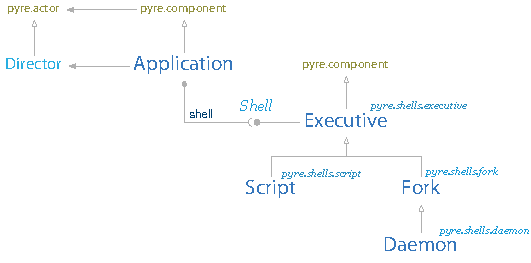
\includegraphics[scale=1.0]{figures/shells.pdf}
  \end{figure}
%
  \item our \identifier{Quad} derives from \identifier{Application}, so it has a
    \identifier{shell}
%
  \end{itemize}
%
\end{frame}

% --------------------------------------
% the parallel version
\begin{frame}[fragile]
%
  \frametitle{Parallel integration}
%
  \begin{itemize}
%
  \item the \identifier{mpi} entry point
%
    \python{firstnumber=36,linerange={36-52}}{listings/quad.py}
%
  \item the \package{mpi} package is part of the pyre distribution
    \begin{itemize}
    \item handles initialization and finalization of \package{MPI}
    \item simplifies most of the ``overhead'' activities
    \item provides an OO veneer
    \end{itemize}
%
  \end{itemize}
%
\end{frame}

% --------------------------------------
% running the mpi program
\begin{frame}[fragile]
%
  \frametitle{Running in parallel}
%
  \begin{itemize}
%
  \item minor modifications to the configuration file...
%
    \cfg{firstnumber=8, linerange={8-28}}{listings/quad.cfg}
%
  \end{itemize}
%
\end{frame}

%-----------------------------------
% end of file


% references
\begin{frame}[allowframebreaks]{references}
  \frametitle{References}
  \bibliographystyle{unsrtnat}
  {\small \bibliography{sections/references}}
\end{frame}

\end{document}

% end of file
